\documentclass[a4paper, 9pt]{report}
\usepackage{pack}

\title{Mathématiques Supérieures\\ Classe de PCSI}

\author{Balthazar Charles}

\pagestyle{empty}

\makeatletter
\def\@makechapterhead#1{%
  %%%%\vspace*{50\p@}% %%% removed!
  {\parindent \z@ \raggedright \normalfont
    \ifnum \c@secnumdepth >\m@ne
        \huge\bfseries \@chapapp\space \thechapter
        \par\nobreak
        \vskip 20\p@
    \fi
    \interlinepenalty\@M
    \Huge \bfseries #1\par\nobreak
    \vskip 40\p@
  }}
\def\@makeschapterhead#1{%
  %%%%%\vspace*{50\p@}% %%% removed!
  {\parindent \z@ \raggedright
    \normalfont
    \interlinepenalty\@M
    \Huge \bfseries  #1\par\nobreak
    \vskip 40\p@
  }}
\makeatother

\begin{document}

%\maketitle

\vspace*{-20em}

\chapter{Logique et vocabulaire ensembliste}

\section*{Ce que dit le programme}

\textit{Ce chapitre regroupe le vocabulaire, les notations et les modes de raisonnement nécessaires aux étudiants pour la conception et la rédaction efficace d’un texte mathématique. Ils doivent être introduits de manière progressive et être acquis en fin de premier semestre. Le programme se limite à une approche naïve des notions d’ensemble et d’application. En particulier, toute étude systématique de la logique ou de la théorie des ensembles est exclue. L’algèbre générale ne figure pas au programme. Plusieurs groupes classiques étant rencontrés en algèbre linéaire, la terminologie associée peut être utilisée mais aucune connaissance théorique sur cette structure n’est exigible.}

\begin{table}[h!]
    \begin{center}
        \begin{tblr}{colspec = {XX}}
            \SetCell{c} \textsc{Contenus} & \SetCell{c} \textsc{Capacités \& commentaires} \\
            \hline
            \SetCell[r=1, c=2]{l} {\color{red} a) Rudiments de logique} & \\
            \hline[.1pt, gray]
            Quantificateurs. & Les étudiants doivent savoir employer les quantificateurs pour formuler de façon précise certains énoncés et leur négation. En revanche, l’emploi des quantificateurs en guise d’abréviations est exclu.\\
            Implication, contraposition, équivalence. &\\
            Modes de raisonnement : raisonnement par récurrence,
            par contraposition, par l’absurde, par analyse-synthèse.&
            Toute construction et toute axiomatique de $\NN$ sont hors
            programme. Le raisonnement par analyse-synthèse est
            l’occasion de préciser les notions de condition nécessaire
            et de condition suffisante\\
            \hline
            \SetCell[r=1, c=2]{l} {\color{red} b) Ensembles} & \\
            \hline[.1pt, gray]
            Appartenance, inclusion. &\\
            Sous-ensembles (ou parties) d’un ensemble, ensemble vide.&\\
            Opérations sur les parties d’un ensemble : réunion, intersection, complémentaire.&
            Notations $\complement_E^A, \overline{A}, E \setminus A$.
            Les étudiants doivent maîtriser le lien entre connecteurs logiques et opérations ensemblistes.\\
            Produit cartésien de deux ensembles, d’un nombre fini d’ensembles.&\\
            Ensemble des parties d’un ensemble.\\
        \end{tblr}
    \end{center}
\end{table}

\begin{table}[h!]   
    \begin{center}
        \begin{tblr}{colspec = {XX}}
            \SetCell{c} \textsc{Contenus} & \SetCell{c} \textsc{Capacités \& commentaires} \\
            \hline
            \SetCell[r=1, c=2]{l} {\color{red} b) Applications et relations d'équivalence} & \\
            \hline[.1pt, gray]
            Application d’un ensemble non vide $E$ dans un ensemble non vide $F$ ; graphe d’une application. 
            & Le point de vue est intuitif : une application de $E$ dans $F$ associe à tout élément de $E$ un unique élément de $F$ . Notations $\mathcal{F}(E,F)$ et $F^E$ pour l’ensemble des applications de $E$ dans $F$.\\
            Famille d’éléments d’un ensemble $E$ indexée par un ensemble fini.\\ Fonction indicatrice d’une partie $A$ d’un ensemble $E$. & Notation $\ind_A$.\\
            Restriction. & Notation $f_{|A}$.\\
            Image directe. & Notation $f(A)$.\\
            Image réciproque. & Notation $f\inv(B)$.\\
            Composition.\\
            Injection, surjection. Composée de deux injections, de deux surjections.\\
            Bijection, réciproque. Composée de deux bijections, réciproque de la composée. \\
            Relation d’équivalence, classes d’équivalence. &La notion d’ensemble quotient est hors programme.\\
            \hline
        \end{tblr}
    \end{center}
\end{table}

\newpage

\section{Rudiments de logique}

%\begin{dftn}
    Une \emph{assertion} ou \emph{proposition} est une phrase logique syntaxiquement correcte, ayant un sens, et dont on peut dire sans ambiguïté si elle est vrai ou fausse. On appelle la vérité ou fausseté d'une assertion sa \emph{valeur de vérité}. 
\end{dftn}

\begin{lined}
    Par exemple, "$x = 2$ et $x > 5$" est une assertion, qui est fausse.
\end{lined}

Le travail du mathématicien consiste à décider, étant donné une assertion, sa valeur de vérité.\footnote{Ce travail est en fait sans espoir. \textit{Cf.} Gödel, Turing, etc.}

\begin{dftn}
    Un \emph{prédicat d'arité $n$}, où $n$ est un entier naturel, est une phrase logique syntaxiquement correcte, qui prend un sens lorsque l'on précise ou quantifie $n$ variables, et dont on peut déterminer la valeur de vérité une fois ces variables préciser.
\end{dftn}

En général, un prédicat porte implicitement sur des variables "d'un certain type", ou vivant dans un certain ensemble. D'une certaine façon, on peut voir un prédicat comme une fonction de cette ensemble vers les assertions.

\begin{lined}
    Par exemple, "avoir un carré supérieur à 5" est un prédicat. Si on le note $P$, on peut, pour tout $x$ réel, considérer l'assertion $P(x)$ : "ce $x$ spécifique a un carré supérieur à 5". Dans ce cas, le prédicat est implicitement défini sur les objets 1)~dont on peut prendre le carré 2)~dont le carré peut être comparé à 5. Autre exemple, les symboles $=, \leq, >$... dénotent des prédicats d'arité 2.
\end{lined}

Étant donné un prédicat défini sur un ensemble, on peut se demander pour quels éléments de cet ensemble le prédicat est vrai.

\begin{dftn}
    Soit $P$ un prédicat défini sur un ensemble $E$. 
    
    On note $\forall x \in E, P(x)$ l'assertion "l'assertion $P(x)$ est vraie quel que soit l'élément $x \in E$". On dit que $\forall$ est le \emph{quantificateur universel} et on le lit "pour tout" où "quel que soit".

    On note $\exists x \in E, P(x)$ l'assertion "l'assertion $P(x)$ est vraie pour au moins un élément $x \in E$". On dit que $\exists$ est le \emph{quantificateur existentiel} et on le lit "il existe".
\end{dftn}

Attention, étant donné un prédicat $P$ définit sur $E$, les assertions $P(x)$ pour $x \in E$ donné, $\forall x \in E, P(x)$ et $\exists x \in E, P(x)$ n'ont aucune raison d'être vraies ou fausses simultanément.

\subsection{Fonctions booléennes}

\begin{dftn}
    On appelle \emph{booléen} les éléments de $\{\mathtt{Vrai}, \mathtt{Faux}\}$. Étant donné un entier naturel $n$, on appelle \emph{fonction booléenne} d'arité $n$, ou à $n$ arguments, une fonction de $\{\mathtt{Vrai}, \mathtt{Faux}\}^n$ à valeur dans $\{\mathtt{Vrai}, \mathtt{Faux}\}$.
\end{dftn}

\begin{lined}
    Pour tout $n \in \NN$, on peut voir $\mathtt{Vrai}$ (respectivement $\mathtt{Faux}$), comme la fonction constante renvoyant toujours $\mathtt{Vrai}$ (resp. $\mathtt{Faux}$).
\end{lined}

\begin{prop}
    Il existe exactement 2 fonctions booléennes à 0 arguments, 4 fonctions booléennes à 1 argument et 16 fonctions booléennes à 2 arguments, et plus généralement $2^{2^n}$ fonctions booléennes à $n$ arguments.
\end{prop}

\begin{proof}
    Pour entièrement déterminer une fonction booléenne d'arité $n$, il faut et il suffit d'associer chaque $\mathtt{Vrai}$ ou $\mathtt{Faux}$ à chaque élément de $\{\mathtt{Vrai}, \mathtt{Faux}\}^n$. Cet ensemble contient $2^n$ éléments, pour chacun desquels deux choix sont possibles. Il y a donc $2^{2^n}$ telles fonctions booléennes.
\end{proof}

Connaissant leur nombre, on peut en lister quelques-unes.

-- \textbf{Arité 0.} $\mathtt{Vrai}, \mathtt{Faux}$

-- \textbf{Arité 1.} $\mathtt{Vrai}, \mathtt{Faux}$ et également :
$$\left\{\begin{aligned}
    \mathtt{Vrai} & \mapsto \mathtt{Vrai}\\
    \mathtt{Faux} & \mapsto \mathtt{Faux}
\end{aligned}\right.,
\qquad\qquad
\left\{\begin{aligned}
    \mathtt{Vrai} & \mapsto \mathtt{Faux}\\
    \mathtt{Faux} & \mapsto \mathtt{Vrai}
\end{aligned}\right..$$
On nomme cette dernière fonction "NON". On la note souvent, étant donné un booléen $A$, par $\overline{A}$ ou encore $\neg A$. On observe facilement que NON est involutif, c'est-à-dire que pour tout booléen $A$, on a $\neg(\neg(A)) = A$.

-- \textbf{Arité 2.} Elles sont trop nombreuses pour que nous les notions toutes ici. Cependant, voyons-en quelques-unes important. On les donne par leur \emph{table de vérité} : ici un tableau à double entrée donnant en colonne la valeur d'un premier booléen $A$ et en colonne celle d'un second booléen $B$. On abrège $\mathtt{Vrai}$ par $\vrai$ et $\mathtt{Faux}$ par $\faux$.
\begin{center}
    \begin{tblr}{X[c]X[c]X[c]|X[c]X[c]X[c]}
        \textsc{Nom} & \textsc{Table} & \textsc{Notation} & \textsc{Nom} & \textsc{Table} & \textsc{Notation}\\
        \hline\hline
        ET & \SetTblrInner{rowsep=0pt}
        \begin{tblr}{c|c|c}
            \diagbox[innerwidth=.5cm]{$B$}{$A$}&$\vrai$&$\faux$\\
            \hline
            $\vrai$&$\vrai$&$\faux$\\
            \hline
            $\faux$&$\faux$&$\faux$
        \end{tblr} & $A$ et $B$, $A \wedge B$
        & OU & \SetTblrInner{rowsep=0pt}
        \begin{tblr}{c|c|c}
            \diagbox[innerwidth=.5cm]{$B$}{$A$}&$\vrai$&$\faux$\\
            \hline
            $\vrai$&$\vrai$&$\vrai$\\
            \hline
            $\faux$&$\vrai$&$\faux$
        \end{tblr} & $A$ ou $B$, $A \vee B$\\
        \hline
        Implication & \SetTblrInner{rowsep=0pt}
        \begin{tblr}{c|c|c}
            \diagbox[innerwidth=.5cm]{$B$}{$A$}&$\vrai$&$\faux$\\
            \hline
            $\vrai$&$\vrai$&$\vrai$\\
            \hline
            $\faux$&$\faux$&$\vrai$
        \end{tblr} & $A \Rightarrow B$
        & Implication réciproque & \SetTblrInner{rowsep=0pt}
        \begin{tblr}{c|c|c}
            \diagbox[innerwidth=.5cm]{$B$}{$A$}&$\vrai$&$\faux$\\
            \hline
            $\vrai$&$\vrai$&$\faux$\\
            \hline
            $\faux$&$\vrai$&$\vrai$
        \end{tblr} & $A \Leftarrow B$\\
        \hline
        Equivalence & \SetTblrInner{rowsep=0pt}
        \begin{tblr}{c|c|c}
            \diagbox[innerwidth=.5cm]{$B$}{$A$}&$\vrai$&$\faux$\\
            \hline
            $\vrai$&$\vrai$&$\faux$\\
            \hline
            $\faux$&$\faux$&$\vrai$
        \end{tblr} & $A \Leftrightarrow B$
        & OU Exclusif & \SetTblrInner{rowsep=0pt}
        \begin{tblr}{c|c|c}
            \diagbox[innerwidth=.5cm]{$B$}{$A$}&$\vrai$&$\faux$\\
            \hline
            $\vrai$&$\faux$&$\vrai$\\
            \hline
            $\faux$&$\vrai$&$\faux$
        \end{tblr} & $A \oplus B$ (rare)
    \end{tblr}
\end{center}

Bien entendu, on peut combiner ces fonctions booléennes, par exemple en $$(A \vee \neg B) \wedge \neg ((A \vee B) \wedge C)$$ où $A, B, C$ sont des variables booléennes. Notez que les parenthèses sont importantes : il existe des conventions sur la priorité d'application des fonctions booléennes, mais elles ne sont pas universelles. Il vaut donc mieux être explicite et parenthéser l'expression aussi clairement que possible. L'exception à ce conseil concerne la fonction NON : on considère qu'elle est la plus prioritaire de toutes. Ainsi, $\neg A \vee B = (\neg A) \vee B$, par exemple.

\begin{lined}
    On remarquera que la même fonction booléenne peut avoir plusieurs \emph{expressions} comme composition d'autres fonctions. Par exemple $A \vee \neg A$ et $\vrai$ sont deux expressions différentes, mais sont égales en tant que fonctions.
\end{lined}

\begin{rlined}
    \begin{exo}[\textsc{Important}]
        À quelle fonction présentée dans le tableau ci-dessus correspond l'expression $\neg A \vee B$ ? Et $\neg B \Rightarrow A$ ?
    \end{exo}
\end{rlined}

\begin{prop}
    Pour tout $n \in \NN$, on peut écrire toute fonction booléenne d'arité $n$ en utilisant uniquement $\vrai, \faux, \wedge, \vee, \neg$.
\end{prop}

\begin{proof}
    On raisonne par récurrence pour prouver que la propriété $P(n)$ : "on peut écrire toute fonction booléenne d'arité $n$ en utilisant uniquement $\vrai, \faux, \wedge, \vee, \neg$" est vraie pour tout $n$. 
    Il est évident que $P(0)$ est vraie. Supposons $P(n)$ et soit $f$ une fonction booléenne d'arité $n+1$. La fonction qui à tout $(b_i)_{1 \leq i \leq n} \in \{\vrai, \faux\}^n$ associe $f(b_1, \dots, b_n, \vrai)$ est une fonction d'arité $n$. Notons là $f_{\vrai}$. De la même façon, on définit une fonction $f_{\faux} = f(\cdot, \dots, \cdot, \faux)$. D'après $P(n)$, il existe deux expressions $E_{\vrai}, E_{\faux}$ en $n$ variables utilisant uniquement $\vrai, \faux, \wedge, \vee, \neg$, telles que $E_{\vrai} = f_{\vrai}$ et $E_{\faux} = f_{\faux}$ en tant que fonction. Alors :
    $$f(b_1, \dots, b_{n+1}) = (E_{\vrai}(b_1, \dots, b_n) \wedge b_{n+1}) \vee (E_{\faux}(b_1, \dots, b_n) \wedge \neg b_{n+1}).$$
    On conclut par le principe de récurrence.
\end{proof}

\subsection{Composition des opérateurs booléens}

À un haut niveau, on peut voir le travail du mathématicien comme la manipulation d'expressions booléennes : partant de résultats connus ou de vérités évidentes, il s'agit de le combiner dans des fonctions booléennes, appelées dans ce contexte \emph{opérateurs logiques}, pour en obtenir de nouveau. Pour raisonner correctement, il est donc nécessaire d'être à l'aise avec ces opérateurs logiques et la façon dont ils se composent les uns avec les autres.

On a déjà vu comment NON se compose avec elle-même : elle est involutive.

\begin{prop}[Lois de De Morgan]
    Pour tous booléens $A, B$, on a $\neg (A \wedge B) = \neg A \vee \neg B$ et $\neg(A \vee B) = \neg A \wedge \neg B$.
\end{prop}

\begin{proof}
    Il est facile de se convaincre que c'est le cas en traduisant les formules logiques en français "si on n'a pas les deux, c'est qu'il manque un des deux" (et réciproquement) et "si on n'a aucun des deux, c'est qu'on a ni l'un ni l'autre". Cependant, on peut avoir une preuve simplement en considérant les tables de vérité.

    \begin{center}
        \begin{tblr}{c|cccc}
            $A$ & $\vrai$ & $\vrai$ & $\faux$ & $\faux$\\
            $B$ & $\vrai$ & $\faux$ & $\vrai$ & $\faux$\\
            $A \wedge B$ & $\vrai$ & $\faux$ & $\faux$ & $\faux$\\
            $\neg(A \wedge B)$ & $\faux$ & $\vrai$ & $\vrai$ & $\vrai$\\
            $\neg A \vee \neg B$ & $\faux$ & $\vrai$ & $\vrai$ & $\vrai$
        \end{tblr}
        \qquad\qquad
        \begin{tblr}{c|cccc}
            $A$ & $\vrai$ & $\vrai$ & $\faux$ & $\faux$\\
            $B$ & $\vrai$ & $\faux$ & $\vrai$ & $\faux$\\
            $A \vee B$ & $\vrai$ & $\vrai$ & $\vrai$ & $\faux$\\
            $\neg(A \vee B)$ & $\faux$ & $\faux$ & $\faux$ & $\vrai$\\
            $\neg A \wedge \neg B$ & $\faux$ & $\faux$ & $\faux$ & $\vrai$
        \end{tblr}
    \end{center}
\end{proof}

Cette manière de présenter les tables de vérité devient plus pratique que la précédente dès que l'on a plus d'une fonction, ou plus de deux variables.

\begin{rlined}
    \begin{exo}(\textsc{Important})\label{exo:bool}
        Montrer à l'aide de tables de vérité les propriétés (à connaitre !) suivantes.
        Pour tous $A, B, C$ booléens :
        \begin{itemize}
            \item $A \wedge B = B \wedge A$ et $A \vee B = B \vee A$ (on dit que ET et OU sont commutatives).
            \item $A\wedge(B\wedge C) = (A\wedge B)\wedge C$ (on dit que ET est associative).
            \item $A\vee(B\vee C) = (A\vee B)\vee C$ (on dit que OU est associative).
            \item $A \wedge (B \vee C) = A \wedge B \vee A \wedge C$ (on dit que ET est distributive sur OU)
            \item $A \wedge (B \vee C) = A \wedge B \vee A \wedge C$ (on dit que ET est distributive sur OU).
            \item $A \vee \neg A = \vrai, A \wedge \neg A = \faux$.
            \item $(A \Rightarrow B) \wedge (B \Rightarrow A) = A \Leftrightarrow B$
        \end{itemize}
    \end{exo}
    \begin{exo}(\textsc{Important})
        Montrer à l'aide de contre-exemples les propriétés suivantes.
        Il existe des $A, B, C$ booléens :
        \begin{itemize}
            \item $A \vee (B \wedge C) \neq (A \vee B) \wedge C$.
            \item $A \Rightarrow (B \Rightarrow C) \neq (A \Rightarrow B) \Rightarrow C$.
        \end{itemize}
    \end{exo}
\end{rlined}

\newpage

\newpage

\section{Ensembles}

Dans cette section, on va parler de (mais pas de tous les) axiomes définissant la théorie des ensembles. Ces axiomes sont hors programme, mais en avoir entendu parler permet de poser une fondation plus solide sur ce qui est "correct" et ce qui ne l'est pas. En théorie des ensembles, on ne manipule que des ensembles. Quand on quantifie sans précision, par exemple $\forall x$ ou $\exists x$, $x$ est seulement supposé être un ensemble.
Pour des raisons fondamentales à un point contrariant, nous ne pouvons pas donner mieux qu'une définition intuitive de la notion d'ensemble. 

\begin{dftn}
    Un \emph{ensemble} $E$ est une collection d'objets, sans ordre ni multiplicité. On  appelle \emph{éléments} les objets appartenant à $x$. On note $x \in E$ si $x$ est un élément de $E$, et $x \notin E$ autrement.
\end{dftn}

% \begin{ax}
%     Si $E, F$ sont deux ensembles, l'assertion "$E = F$" est vrai si et seulement si $\forall x, x \in E \Leftrightarrow X \in F$.
% \end{ax}

On peut écrire un ensemble de deux façons :
\begin{itemize}
    \item en \emph{extension}, en écrivant tous ses éléments, entre accolades, séparé par des virgules.
    \begin{lined}
        Les ensembles $\{0,1,2\}, \{2,0,1\}$ et $\{2,2,1,0,1\}$ sont le même ensemble. $\{\NN\}$ est également un ensemble. Il n'a qu'un seul élément, on dit que c'est un singleton. $\{\}$, aussi noté $\emptyset$, existe et est l'unique ensemble qui n'a aucun élément. On l'appelle l'\emph{ensemble vide}.
    \end{lined}
    Il est évident qu'il est difficile d'écrire des ensembles trop gros de cette façon.
    \item en \emph{compréhension}, étant donné un ensemble $E$ et un prédicat $P$ défini sur $E$, on peut former $\{x \in E\sepp P(x)\}$, l'ensemble des éléments de $E$ tels que $P(x)$ est vraie. Dans le cas particulier où $f$ est une fonction de $E$ dans $F$, on note plus simplement $\{f(y) \sepp y \in E\}$ plutôt que $\{x \in F \sepp \exists y \in E, x = f(y)\}$.
    \begin{lined}
        $\{2^k \sepp k \in \NN\}$ est l'ensemble des puissances positives de 2. $\{x \in \RR \sepp \cos(x) = 0\}$ est l'ensemble des solutions de l'équation $\cos(x) = 0$.
    \end{lined}
\end{itemize}

La possibilité d'écrire les ensembles de cette façon est assurée par des axiomes, notamment \emph{de la paire} et \emph{de l'union} pour l'extension, et par le \emph{schéma d'axiomes de compréhension} pour la compréhension. Leur définition non ambiguë est affirmée par l'axiome d'\emph{extensionnalité}.

% \begin{ax}[Paire]
%     Si $E, F$ sont des ensembles, il existe un ensemble $G$ tel que $$x \in G \Rightarrow x = E \vee x = F.$$
% \end{ax}

% \begin{ax}[Union]
%     Si $E$ est un ensemble, il existe un ensemble $F$, appelé l'\emph{union} de $E$, noté $\bigcup E$, tel que $$\forall x, x \in F \Leftrightarrow (\exists G \in E, x \in G).$$
% \end{ax}



\begin{dftn}
    On appelle \emph{cardinal} d'un ensemble fini $E$ le nombre de ses éléments. Les notations $|E|$ et $\#E$ sont généralement acceptées pour dénoter le cardinal de $E$.
\end{dftn}

Le prototype de l'ensemble de cardinal $n$, $n \in \NN$ donné, est l'ensemble $\{m \in \NN \sepp 1 \leq n \leq n\}$, noté $\intint{1, n}$. En fait, on le verra plus tard, on définit plus proprement le cardinal d'un ensemble fini $E$ comme étant l'unique entier $n$ tel que $E$ et $\intint{1, n}$ sont en \emph{bijection}.
Plus généralement, pour $a, b$ entiers relatifs avec $a\leq b$, on note $\intint{a, b}$ l'ensemble des entiers entre $a$ et $b$, de cardinal $b-a+1$.

\begin{dftn}
    Soient $E, F$ deux ensembles.
    \begin{itemize}
        \item Si pour tout $x, x \in E$ entraine $x\in F$, on dit que $E$ est inclus dans $F$, ou que $E$ est une \emph{partie} de $F$. On note $E \subset F$.
        \item Deux ensembles sont \emph{égaux} s'ils ont les mêmes éléments : $\forall x \in E, x \in E \Leftrightarrow x \in F$ (assertion dont la vérité  est bien sûr équivalente à celle de $\forall x \in F, x \in E \Leftrightarrow x \in F$). On note $E = F$.
    \end{itemize}
\end{dftn}

"\^Etre inclus" est, comme $=$, un prédicat binaire. Étant donné trois ensembles $A, B, C$, l'assertion $A \subset B \subset C$, évaluée "naturellement" de la gauche vers la droite, n'a \emph{a priori} pas de sens. Cependant, pour signifier $(A \subset B)\wedge(B \subset C)$, on commet l'abus de notation $A \subset B \subset C$.

\begin{lined}
    Pour tout ensemble $E$, $\emptyset \subset E$. En effet, $\forall x \in \emptyset, x\in E$.
\end{lined}

Il est également clair que $E = F \Leftrightarrow E \subset F \wedge F \subset F$. Ainsi, pour montrer l'égalité de deux ensemble on raisonne souvent par  \emph{double inclusion} plutôt qu'en montrant qu'un objet est dans le premier ensemble si et seulement si il est dans le second. Les deux modes de raisonnement sont néanmoins valides : comme partout on choisit celui qui rend la démonstration agréable.

\begin{rlined}
    Attention, être inclus et être un élément n'est pas \emph{du tout} la même chose. L'ensemble vide est inclus dans $\{1, 2, 3\}$, mais n'en est pas un élément. De même $\pi \in \RR$, mais $\{\pi\} \notin \RR$. Dans la même veine, $\{3\}$ n'est pas la solution de l'équation $x = 3$, mais l'\emph{ensemble de ses solutions}.
\end{rlined}

\begin{ax}
    Si $E$ est un ensemble, il existe un ensemble $F$ tel que $x \in F \Leftrightarrow x \subset E$. On l'appelle l'\emph{ensemble des parties} de $E$ et on le note $\mathfrak{P}(E)$, ou parfois $2^E$.
\end{ax}

\begin{lined}
    L'ensemble des parties $\{1, 2, 3\}$ est $\{\emptyset, \{1\}, \{2\}, \{3\}, \{1, 2\}, \{2, 3\}, \{1, 2\}, \{1, 2, 3\}\}$.
\end{lined}

\subsection{Opérations sur les ensembles.}

\begin{dftn}
    Soient $E$ et $F$ deux ensembles. Il existe un ensemble $G$, noté $E \cup F$, appelé l'\emph{union} de $E$ et $F$, tel que $\forall x, x \in G \Leftrightarrow (x \in E \vee x \in F)$.
    
    Si $(E_i)_{i\in I}$ est une famille (possiblement infinie) d'ensembles indexée par un ensemble $I$, il existe un ensemble $G$ vérifiant $\forall x, x\in G \Leftrightarrow \exists i \in I, x\in E_i$. On note $\bigcup_{i\in I} E_i$ cette union.
\end{dftn}

On donne ici l'union d'une famille d'ensemble comme définition, mais en fait, l'existence de l'ensemble union est axiomatique (elle est affirmée par le bien nommé \emph{axiome de l'union}). En général, on ne peut pas démontrer que cette union existe à partir de rien, on \emph{décide} qu'elle existe.

\begin{dftn}
    Soient $E$ et $F$ deux ensembles. L'ensemble $\{x \in E \sepp x \in F\}$ (ou, de façon équivalente $\{x \in F \sepp x \in E\}$) est noté $E \cap F$ et est appelée l'\emph{intersection} de $E$ et $F$. 
        
    On note $\bigcap_{i \in I} E_i$ l'intersection d'une famille (possiblement infinie) d'ensembles indexée par un ensemble $I$, c'est-à-dire l'ensemble $\{x \in \bigcup_{i\in I}E_i \sepp \forall i \in I, x \in I\}$.
\end{dftn}

Pourquoi ce bizarre "$x \in \bigcup_{i\in I}E_i$" dans l'expression de l'intersection ? Parce que lorsqu'on écrit un ensemble en compréhension, il faut préciser d'où on tire les éléments et comme l'intersection est toujours incluse dans l'union (s'en convaincre), on peut les tirer de l'union. Comme on a également $\forall j \in I$, $\bigcap_{i\in I}E_i \subset E_j$, on aurait pu aussi choisir un des $E_i$ et prendre les $x$ dedans... si on accepte l'axiome \emph{du choix}\footnote{et on l'accepte !}.

\begin{rlined}
    \begin{exo}
        Montrer que pour tous ensembles $A, B$, $A \subset B \Leftrightarrow A \cap B = A$ et que $A \subset B \Leftrightarrow A \cup B = B$
    \end{exo}
\end{rlined}

\begin{dftn}
    Soient $E, F$ deux ensembles.
    \begin{itemize}
        \item L'ensemble $\{x \in E \sepp x \notin F\} \cup \{x \in F \sepp x \notin E\}$ est appelé la \emph{différence symétrique} de $E$ et $F$. On la note $E \Delta F$.
        \item Supposons que $E \subset F$. Le \emph{complément} de $E$ dans $F$ est l'ensemble $\{x \in F \sepp x \notin E\}$. On le note $F \setminus E$ (lire dans ce cas "$F$ privé de $E$") ou $\complement_F^E$. Si l'identité de $F$ est claire en contexte, on note parfois aussi $\overline{E}$.
    \end{itemize}
\end{dftn}

Pour le plus grand malheur des mathématiciens de tous âges, on n'a pas beaucoup de symboles vraiment différents et faciles à écrire. Ainsi, on trouve souvent écrit $F \setminus E = \{x \in F \sepp x \notin E\}$, \emph{sans l'hypothèse que $E \subset F$}. On appelle cela le \emph{complémentaire relatif} de $E$ dans $F$. Dans la suite de ce chapitre, on ne parlera de complémentaire que dans le cas d'inclusion. Heureusement, comme pour tous ensembles $E, F$ on a $F \setminus E = F \setminus (F \cap E)$, il est facile de passer d'un cas à l'autre.

\begin{rlined}
    \begin{exo}
        Montrer que $\forall E, \forall F, E\Delta F = F\Delta E$.
    \end{exo}
    \begin{exo}
        Soient $E, F$ des sous-ensembles d'un ensemble $G$. Montrer que $$(E \cap F = \emptyset \wedge E \cup F = G) \Rightarrow E = \overline{F}.$$
    \end{exo}
\end{rlined}

\begin{dftn}
    \begin{itemize}
        \item Soient $E, F$ des ensembles. Si $E \cap F = \emptyset$, on dit qu'ils sont \emph{disjoints}. On dit que leur union est une \emph{union disjointe} et on le signifie en notant $E \sqcup F$. De même, si une famille $(E_i)_{i\in I}$ indexée par un ensemble $I$ vérifie
        $$\forall i \in I, \forall j \in I, i \neq j, E_i \cap E_j = \emptyset,$$
        on note leur union $\bigsqcup_{i\in I}E_i$.
        \item Soit $F$ un ensemble et $(E_i)_{i\in I}$ une famille d'ensembles indexée par un ensemble $I$ telle que $F = \bigsqcup_{i\in I}E_i$. On dit que la famille $(E_i)_{i\in I}$ est un \emph{recouvrement disjoint} de $F$. Sous l'hypothèse supplémentaire qu'aucun des $E_i$ n'est vide, on parle de \emph{partition} de $F$.
    \end{itemize}
\end{dftn}

\begin{lined}
    Par exemple, $\{E \in \mathfrak{P}(\NN) \sepp \#E = 1\}$ est une partition de $\NN$. \'Etant donné un ensemble fini $E$ de cardinal $n$, $\{\{F \subset E \sepp \#F = k\} \sepp k \in \intint{0, n}\}$ est une partition de $\mathfrak{P}(E)$.
\end{lined}

\newpage

\subsection{Lien avec la logique et compatibilité des opérations.}
\label{sets_log}

Il ne vous aura pas échappé que les opérations ensemblistes ont un comportement suspicieusement similaire à celui de la logique booléenne, au point où l'on note le complément et la négation de la même façon. Voyons les correspondances avec les autres connecteurs logiques.

Dans ce paragraphe \ref{sets_log}, $E,F,G$ désignent, une bonne fois pour toutes, des ensembles. On suppose également que $E, F$ sont des sous-ensembles de $G$. On y note $x$ un élément quelconque de $G$.

\begin{table}[h!]
    \begin{tblr}{X[c,m]X[c,m]X[c,m]X[2,c,m]}
        \textsc{Opération ensembliste} & \textsc{Propriété définissant les éléments} & \textsc{Opération logique correspondante} & \textsc{Patates}\\
        \hline\hline
        $E \cap F$ & $x \in E \wedge x \in F$ & $\wedge$ & 
        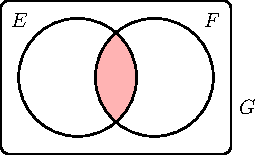
\includegraphics[align = c]{./figures/cap.pdf}\\
        $E \cup F$ & $x \in E \vee x \in F$ & $\vee$ & 
        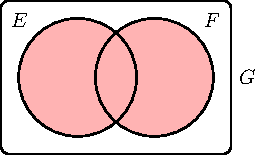
\includegraphics[align = c]{./figures/cup.pdf}\\
        $G \setminus F$ & $\neg(x \in F)$ & $\neg$ (presque) & 
        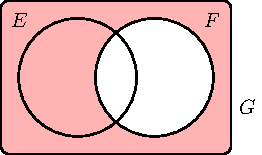
\includegraphics[align = c]{./figures/neg.pdf}\\
        $E \Delta F$ & $x \in E \oplus x \in F$ & $\oplus$ (ou exclusif) & 
        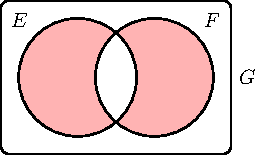
\includegraphics[align = c]{./figures/xor.pdf}\\
        $G \setminus (E \Delta F)$ & $x \in E \Leftrightarrow x \in F$ & $\Leftrightarrow$ & 
        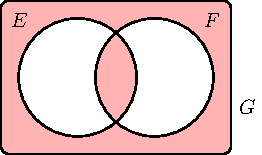
\includegraphics[align = c]{./figures/equiv.pdf}\\
    \end{tblr}
    \caption{Correspondance entre opérateurs logiques et opérations ensemblistes.}
    \label{tab:log=ens}
\end{table}

\newpage

Notons que, contrairement au cas de la logique "pure", on a besoin d'un contexte pour le complémentaire : $\NN \setminus \{1, 2, 3\}$ existe, mais l'ensemble contenant tous les objets possibles sauf ceux de $\{1, 2, 3\}$ n'existe pas. En contraste, le prédicat $\notin \{1,2,3\}$ est bien défini pour tous les objets (on peut toujours, au moins en théorie, tester l'appartenance à un ensemble). Si on choisit de se restreindre au cas, souvent suffisant, où le prédicat est défini sur un ensemble, les deux notions redeviennent équivalentes.

On peut également voir l'implication comme une assertion ensembliste : si $P$ et $Q$ sont des prédicats définis sur $G$, $P$ implique $Q$, si et seulement si $\{x \in G \sepp P(x)\} \subset \{x \in G \sepp Q(x)\}$. Ainsi, le raisonnement par double inclusion est l'analogue ensembliste du raisonnement par double implication.

\begin{rlined}
    \begin{exo}[\textsc{Fait en cours}]
        Soient $a, b$ des réels tels que $a \leq b$. Montrer que $[a, b] = \{ta+(1-t)b\sepp t \in [0, 1]\}$. 
    \end{exo}
    \begin{exo}[\textsc{Important}]
        Montrer les propriétés suivantes.
        \begin{itemize}
            \item $E \cap \emptyset = \emptyset, E\cup\emptyset = E, E\cap G = E, E\cup G = G$.
            \item $E \cap F = F \cap E$ et $E \cup F = F \cup E$.
            \item $(E \cap F) \cap G = E \cap (F \cap G)$ et $(E \cup F) \cup G = E \cup (F \cup G)$.
            \item $(E \cap F) \cup G = (E \cup G) \cap (F \cup G)$ et $(E \cup F) \cap G = (E \cap G) \cup (F \cap G)$.
            \item Si $E \subset G$, $(G \setminus (G \setminus E)) = E$.
            \item Si $E, F$ sont des parties de $G$, $G \setminus (E \cap F) = (G \setminus E) \cup (G \setminus F)$.
            
            et $G \setminus (E \cup F) = (G \setminus E) \cap (G \setminus F)$.
        \end{itemize}
    \end{exo}
\end{rlined}

On doit être capable de montrer formellement ces propositions, mais on peut facilement s'en convaincre par un dessin. Par exemple :
\begin{table}[h!]
    \begin{tblr}{X[c,m]cX[c,m]cX[c,m]}
        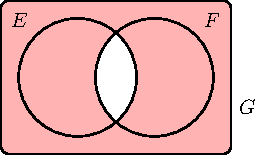
\includegraphics[align = c]{./figures/negcap.pdf} 
        & $=$ & 
        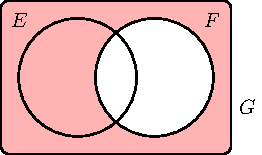
\includegraphics[align = c]{./figures/neg.pdf} 
        & $\cup$ &
        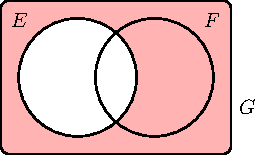
\includegraphics[align = c]{./figures/negF.pdf} \\
    \end{tblr}
\end{table}

Évidemment, ces propriétés s'adaptent quand on fait une intersection ou une union sur une famille quelconque. Prouvons, pour la pratique, la propriété suivante.

\begin{prop}
    Soit $(E_i)_{i\in I}$ une famille d'ensembles indexée par $I$ et $F$ un ensemble. On a $(\bigcap_{i\in I} E_i)\cup F = \bigcap_{i\in I} (E_i \cup F)$.
\end{prop}

\begin{proof}
    Pour tout $x$, on a :
    \begin{align}
        x \in (\bigcap_{i\in I} E_i)\cup F & \Leftrightarrow x \in F \vee (\forall i \in I, x \in E_i)\\
        & \Leftrightarrow \forall i \in I, (x \in F \vee x \in E_i) \\
        & \Leftrightarrow x \in \bigcap_{i\in I} (E_i \cup F)
    \end{align}
\end{proof}

En fait, énervons-nous. Pour nous habituer aux techniques, prouvons la proposition \ref{exo:germain}. Elle n'est pas très utile, mais sa preuve constitue un bon entrainement.
\begin{prop}\label{exo:germain}
    Soit $I$ un ensemble et soient $(E_i)_{i \in I}, (F_i)_{i \in I}$. On a :
    $$\bigcup_{i \in I}(E_i \cap F_i) = \bigcap_{X \in \mathfrak{P}(I)}\left(\bigcup_{i \in X} E_i \cup \bigcup_{i \in I \setminus X} F_i\right).$$
\end{prop}

\begin{proof}
    Faite en cours.
\end{proof}

\subsection{Fonction indicatrice}

Dans ce paragraphe, $E, F, G$ sont des ensemble et $E \subset G$.

\begin{dftn}
   La \emph{fonction indicatrice} de $E$ est la fonction à valeurs réelles, définie sur $G$, notée $\ind_E$, donnée par :
   $$\forall x \in F, f(x) = \left\{\begin{aligned}
    1& \textrm{ si } x \in E\\
    0& \textrm{ sinon}
   \end{aligned}\right.$$
\end{dftn}

\begin{prop}
    \begin{itemize}
        \item $\ind_{G \setminus E} = 1 - \ind_E$.
        \item $\ind_{E \cap F} = \ind_E\cdot\ind_F$.
        \item $\ind_{E \cup F} = \max(\ind_E, \ind_F) = \ind_E + \ind_F - \ind_E \cdot \ind_F$.
    \end{itemize}
\end{prop}

\begin{proof}
    Faite en cours.
\end{proof}

\begin{rlined}
    \begin{exo}
        Utiliser ces propriétés pour générer les tables de vérités de l'exercice \ref{exo:bool} à l'aide d'un tableur (LibreOffice Calc, par exemple).
    \end{exo}
\end{rlined}

\subsection{Produit cartésien}

Considérons deux ensembles $E, F$. On peut écrire, en extension, $\{E\}$ et $\{E, F\}$, puis $\{\{E\}, \{E, F\}\}$. Cette manière de faire a un avantage : on gagne une idée d'ordre entre les parties de $\{\{E\}, \{E, F\}\}$ (l'une est inclus dans l'autre, mais pas réciproquement). 

\begin{dftn}
    Soient $E, F$ deux ensembles. Le \emph{produit cartésien} de $E$ et $F$, noté $E \times F$, est l'ensemble 
    $$\{X \in \mathfrak{P}(\mathfrak{P}(E \cup F)) \sepp \exists x \in E, \exists y \in F, X = \{\{x\}, \{x, y\}\}\}.$$
    On appelle les éléments de $E \times F$ des \emph{couples}. 
\end{dftn}

On peut itérer cette construction et obtenir ainsi des triplets, quadruplets... $n$-uplets pour tout $n$ entier naturel.
Cette construction formelle est hors programme, on demande seulement de connaitre la définition intuitive suivante :

\begin{dftn}
    Soit $n$ un entier supérieur ou égal à 2 et $E_1, E_2, \dots, E_n$ des ensembles. Le \emph{produit cartésien} de $E_1, E_2, \dots, E_n$ est l'ensemble des listes ordonnées $(x_1, x_2, \cdot, x_n)$ avec, pour tout $i \in \intint{1, n}, x_i\in E_i$. On le note $E_1\times E_2 \times ... \times E_n$, ou $E^n$ si tous les $E_i$ sont le même ensemble~$E$.
\end{dftn}

Par convention, on décide que $E^1 = E$ et que $E^0 = \emptyset$.

\begin{figure}[h!]
    \begin{center}
        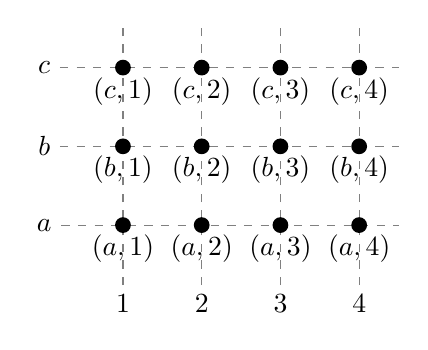
\begin{tikzpicture}
            \node (a) at (-1, 0) {$a$};
            \node (b) at (-1, 1) {$b$};
            \node (c) at (-1, 2) {$c$};
            \node (1) at ( 0,-1) {$1$};
            \node (2) at ( 1,-1) {$2$};
            \node (3) at ( 2,-1) {$3$};
            \node (4) at ( 3,-1) {$4$};

            \draw[dashed, gray] (a) -- (3.5, 0);
            \draw[dashed, gray] (b) -- (3.5, 1);
            \draw[dashed, gray] (c) -- (3.5, 2);
            \draw[dashed, gray] (1) -- ( 0,2.5);
            \draw[dashed, gray] (2) -- ( 1,2.5);
            \draw[dashed, gray] (3) -- ( 2,2.5);
            \draw[dashed, gray] (4) -- ( 3,2.5);

            \fill (0,0) circle (0.1);
            \fill (0,1) circle (0.1);
            \fill (0,2) circle (0.1);
            \fill (1,0) circle (0.1);
            \fill (1,1) circle (0.1);
            \fill (1,2) circle (0.1);
            \fill (2,0) circle (0.1);
            \fill (2,1) circle (0.1);
            \fill (2,2) circle (0.1);
            \fill (3,0) circle (0.1);
            \fill (3,1) circle (0.1);
            \fill (3,2) circle (0.1);

            \node[below] at (0,0) {$(a, 1)$};
            \node[below] at (0,1) {$(b, 1)$};
            \node[below] at (0,2) {$(c, 1)$};
            \node[below] at (1,0) {$(a, 2)$};
            \node[below] at (1,1) {$(b, 2)$};
            \node[below] at (1,2) {$(c, 2)$};
            \node[below] at (2,0) {$(a, 3)$};
            \node[below] at (2,1) {$(b, 3)$};
            \node[below] at (2,2) {$(c, 3)$};
            \node[below] at (3,0) {$(a, 4)$};
            \node[below] at (3,1) {$(b, 4)$};
            \node[below] at (3,2) {$(c, 4)$};

        \end{tikzpicture}
    \end{center}
    \caption{Exemple : produit cartésien de $\{a,b,c\}$ et $\{1,2,3,4\}$.}
\end{figure}
Maintenant que nous connaissons la définition de produit cartésien, on peut définir proprement le terme de "famille indexée par", que l'on a déjà beaucoup utilisée.

\begin{dftn}
    Soit $E, I$ deux ensembles. On appelle \emph{famille indexée par $I$} toute partie $F$ du produit cartésien $I \times E$ tel que pour tout \emph{index} $i$, il existe une unique \emph{valeur} $x \in E$ tel que $(i, e) \in F$.\footnote{En passant, on appelle aussi ça une \emph{fonction} définie sur $I$, mais on en reparlera}
\end{dftn}

La condition signifie simplement qu'il faut que chaque index serve ("pour tout...") et qu'il ne serve qu'une seule fois ("une unique..."). On peut voir ça comme accrocher une petite décoration venue de $I$ aux éléments de $E$ pour ne pas les confondre au cas on voudrait avoir plusieurs fois le même élément (comme des décorations de verre dans une soirée).

\subsection{Quelques notations habituelles}

Les notations précédentes sont en grande partie déjà apparues.

\begin{itemize}
    \item $\NN$ est l'ensemble des nombres entiers naturels.
    \item $\ZZ$ est l'ensemble des nombres entiers relatifs.
    \item $\QQ$ est l'ensemble des nombres rationnels.
    \item $\RR$ est l'ensemble des nombres réels.
    \item $\CC$ est l'ensemble des nombres complexes.
    \item On note $\NN^*, \ZZ^*, \QQ^*, \RR^*, \CC^*$ pour désigner les ensembles précédents privés de $0$. Attention, cette notation est réservée pour ces ensembles spéciaux.
    \item On note $\QQ^+, \QQ^-, \RR^+, \RR^-$ les sous-ensembles des nombres positifs et négatifs de $\QQ$ et $\RR$. On peut aussi note $\QQ^{+*}, \RR^{-*}$... Dans ces derniers cas de figures, on trouve parfois la notation $\QQ_-^*, \RR_+^*$... plus harmonieuse.
    \item Si $a, b \in \RR$, avec $a<b$, on note $[a, b] = \{x \in \RR \sepp a \leq x \leq b\}$. On appelle cet ensemble le \emph{segment} de $a$ à $b$.
    \item Si $a, b \in \RR$, avec $a<b$, on note $]a, b] = \{x \in \RR \sepp a < x \leq b\}$. On appelle cet ensemble l'\emph{intervalle ouvert en $a$, fermé en $b$}. On définit de même $[a, b[$, l'\emph{intervalle fermé en $a$, ouvert en $b$}.
    \item Si $a, b \in \RR$, avec $a<b$, on note $]a, b[ = \{x \in \RR \sepp a < x < b\}$. On appelle cet ensemble l'\emph{intervalle ouvert} de $a$ à $b$.
\end{itemize}

\end{document}